\subsection{Sensors block}\label{chapter_SENSORS_BLOCK}
The first important hint in this chapter is, that the input is on the right side of the model, because the sensors are in the backward line of the closed loop in figure \ref{fig:MATLAB Overview} (green block).
\begin{figure}[H]
	\centering
		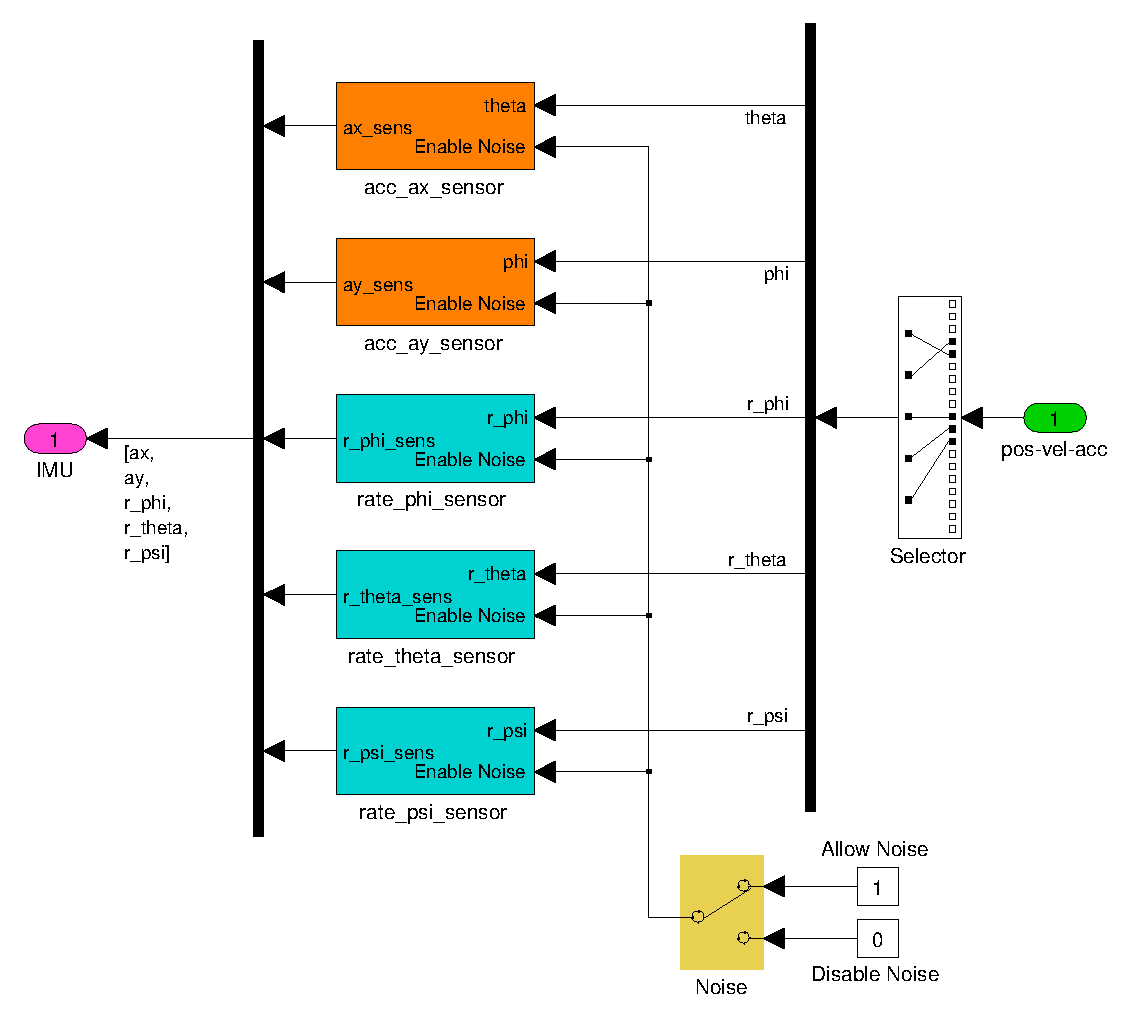
\includegraphics[width=0.9\textwidth]{03_Grafiken/MATLAB_Sensors.pdf}
	\caption{Sensors block}
	\label{fig:Sensors block}
\end{figure}
The first block after the input is a line-selector, that picks the elements out of the \textit{pos\_vel\_acc}-vector, that get measured in the real copter by the sensors. These values are the inputs of each sensor. The upper, orange blocks represent the linear acceleration sensors, that measure the accelerations in direction of \textit{x} and \textit{y} of the bodyframe. These accelerations are not contained in the \textit{pos\_vel\_acc}-vector. So, they have to be calculated in the (model of the) sensor, using the angle and a trigonometric function.
The angular velocities are included in the output vector of the dynamics block, so they get directly 'measured' by the sensors. All measured values are combined in the output vector \textit{IMU} of the sensors block. 